\section{Light blocking (Photo-interrupter) module}
\begin{figure}[H]
    \centering
    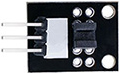
\includegraphics[angle=0, keepaspectratio=true, scale=1, width=200px, height=200px]{images/light_blocking.jpg}
    %\caption{Caption}
\end{figure}
\subsection*{Description}
The photo-interrupter module contains an infrared LED and photo-transistor designed to detect an object in the gap. As the module uses infrared it can detect even transparent objects in the gap.
\subsection*{Pin mapping}
This pin mapping corresponds to the pins from left to right with the module pins facing towards you.
\begin{table}[H]
    \centering
    \begin{tabular}{|c|c|c|c|c|}
    \hline
    Index &Label &Type &Name &Description\\ \hline
    0 &- &Ground &GND &\\ \hline
    1 & &Source voltage &$V+$ &Module source voltage ($5V$)\\ \hline
    2 &S &Analog output &A0 &\\ \hline
    \end{tabular}
    %\caption{Caption}
    %\label{tab:my_label}
\end{table}
\subsection*{Operation}
The output voltage at the analog output pin (A0) is low when the gap is empty. When an object enters the gap the output of A0 will increase until the object has filled the gap at which point the output will be high.
\subsection*{Code}
Refer to listing \ref{python_lightblocking}.
%\lstinputlisting[caption=test]{laser.py}